\documentclass[border=3pt,tikz]{standalone}
\usepackage{amsmath}
\usetikzlibrary{calc}
\usetikzlibrary{arrows.meta} % for arrow size
\begin{document}
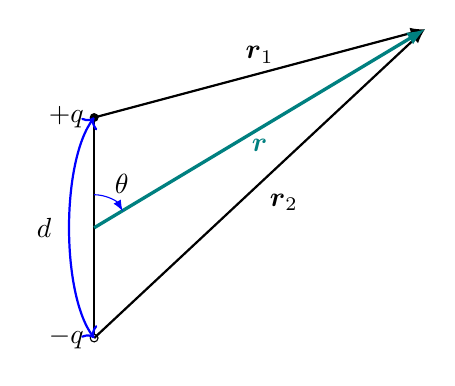
\begin{tikzpicture}[scale=1.4, rotate=0]
    
    \coordinate (O) at (0, 0);
    \coordinate (P1) at (0, 1);
    \coordinate (P2) at (0, -1);
    \coordinate (R) at (3, 1.8);
    \draw [thick] (O) -- (P1) node [left] {$+q$};
    \draw[black,fill=black] (P1) circle (1pt);
    \draw [thick] (O) -- (P2) node [left] {$-q$};
    \draw[black,fill=white] (P2) circle (1pt);
    \draw[thick, -latex] (P1) -- node [above] {$\boldsymbol{r}_1$} (R);
    \draw[thick, -latex] (P2) -- node [below right] {$\boldsymbol{r}_2$} (R);
    \draw[very thick, teal, -latex] (O) -- node [below] {$\boldsymbol{r}$} (R);
    \draw[blue, -latex] (0, 0.3) arc (90:30:0.3);
    \node [right] at (0.1, 0.4) {$\theta$};
    \draw[thick,blue,<->] (P1) .. controls (-0.3, 0.6) and (-0.3, -0.6)  .. (P2);
    \node [left] at (-0.3, 0.0) {$d$};
  \end{tikzpicture}
\end{document}